\begin{tikzpicture} 
\begin{axis}[
axis lines*=middle,
enlargelimits = true,
ymin=-1.2,
ymax=1.2,
xmin=0,
xmax=10,
axis line style={->,>=stealth},
%xlabel={\Large $n$},
%ylabel={\Large $x[n]$},
yticklabel style = {yshift=0.2cm},
xticklabel style = {yshift=-0.1cm},
every axis x label/.style={
    at={(ticklabel* cs:1)},
    anchor=north,
},
every axis y label/.style={
    at={(ticklabel* cs:1)},
    anchor=south,
},
%xtick=\empty,
ytick=\empty,
xtick=\empty,
every outer y axis line/.append style={white!15!black},
every y tick label/.append style={font=\color{white!15!black}},
legend style={draw=white!15!black,fill=white,legend cell align=left}]

\only<1|handout:1>{
\addplot[smooth, line width=1.5pt, domain=0:10, samples=101] {cos(deg(2*pi*0.75*x))};
}

\only<2-|handout:1>{
\addplot[smooth, black!50, line width=1.5pt, domain=0:10, samples=101] {cos(deg(2*pi*0.75*x))};
\addplot[ycomb, mark=*, fill=white, mark options={scale=1.5, fill=white}, line width=1.5pt, domain=0:10, samples=11] {cos(deg(2*pi*0.75*x))};
}

\only<3-|handout:1>{
\addplot[smooth, red, line width=1.5pt, domain=0:10, samples=51] {cos(deg(2*pi*0.25*x))};
}

\end{axis}
\end{tikzpicture}
